\documentclass[11pt, oneside]{report} 

% margins
\usepackage[top=1in, bottom=1.25in, left=1in, right=1in]{geometry} 

\usepackage{titlesec}


\usepackage{graphicx}
\graphicspath{ {images/} }												\usepackage{amssymb}

% Define "align" environment used in demo-mathematics.tex.
\usepackage{amsmath}

% Define "multicols" environment environment used in demo-multicols.tex.
\usepackage{multicol}

% Define "subfigure" environment used in "demo-figure.tex".
%\usepackage{subfigure}
\usepackage{cite}
\usepackage[utf8]{inputenc}

% paragraph indent
\setlength{\parindent}{2em}

% paragraph spacing
\setlength{\parskip}{1em}

% caption fontsize
\usepackage[font={small}, labelfont={bf}]{caption}
\usepackage{float}

% adjusting size of table
\usepackage{adjustbox,lipsum}

% push footnotes to bottom
\usepackage[bottom]{footmisc}

% sub images
\usepackage{subcaption}

\usepackage{hyperref}
\hypersetup{
    colorlinks,
    citecolor=black,
    filecolor=black,
    linkcolor=black,
    urlcolor=black
}


%SetFonts

%SetFonts


\title{\textsc{\textbf{Ambulatory Gait Analysis}}\\ \vspace{5mm} \Large{Clinical Applications and Technical Considerations}
}

\author{Jenna Blumenthal}
%\date{}							% Activate to display a given date or no date

\renewcommand*\contentsname{Table of Contents} % change TOC title
\begin{document}
\bibliographystyle{plain}
\maketitle
\renewcommand{\vspace}[2]{}% Gobble 2 arguments after \vspace
\tableofcontents

\pagebreak

\section*{Introduction}
\addcontentsline{toc}{section}{\textsc{\textbf{Introduction}}} % add to TOC

The purpose of this literature review is to give an overview of gait assessment and how it is used in clinical evaluation. Currently, gait analysis is most often used to provide an objective evaluation of motor impairment, or effectiveness of rehabilitation treatments. However functional assessment is only a small role that quantitative gait analysis can play. If the definition of gait analysis is expanded to include interpreting the significance of quantitative gait data, then the most promising area of gait analysis is ultimately to understand the complex relationship between physical and cognitive impairment, functional disability and gait dysfunction\cite{JoelA.DeLisa1998}.

A limiting factor in the use of gait analysis as a clinical marker may be that data has been traditionally collected using expensive and complicated tools. However with growing penetration of smartphone systems and wearable sensors in healthcare, critical physiologic metrics that were once only possible to be measured in a clinical setting can now be measured during routine activities with a level of accuracy and continuity that could previously only be found in intensive care units. These technologies increase our ability to monitor these metrics in a patient's natural environment, and understand the variability inherent to the individual.

The first section of this review will briefly outline the mechanics and neurologic control of human gait, clinical utility of gait analysis and the current measurement methods. The next section will explore the use of wearable sensors for gait analysis. Technical requirements and usability engineering concerns in healthcare technology design will also be presented. Finally, a summary of work done to date with be given.

\pagebreak

\chapter{Clinical Utility of Gait Analysis}

\section{Human Gait}

\subsection{The Gait Cycle}

In non-pathologic conditions, human walking is a repetitive, periodic movement of body segments. The gait cycle has been broadly divided into two phases: stance phase and swing phase, and these phases can be further subdivided and discussed in terms of percentage of each within the gait cycle\cite{Tao2012}. The gait cycle can be defined as the time interval or sequence of motion occurring from heelstrike to heelstrike of each foot. Though this terminology has been conventionally used as the critical actions of separated gait phases, it is important to note that so called `normal' gait events may fail to accommodate the deviations of gait-impaired patients\cite{Tao2012}. For instance, the heel of a paralytic patient may never be in contact the ground or may do so significantly later in the gait cycle. Similarly, initial floor contact may be made by the entire foot (flat foot), rather than having forefoot contact, which occurs later, after a period of heel-only support\cite{Tao2012}.

As illustrated in Figure \ref{fig:gait_cycle}, the stance phase represents $\sim$60\% of the gait cycle, and can be further divided into double support and single support. In double support, both feet are in contact with the ground. The time spent in double support phase decreases as walking speed increases, and ultimately disappears when one begins to run. The muscle active during the stance phase act to prevent buckling of the support limbs.

The swing phase is described when the limb is not weight bearing, and represents $\sim$40\% of the gait cycle. It can be subdivided into three phases: initial swing (acceleration), midswing, and terminal swing (deceleration). 

\begin{figure}
  \centering
    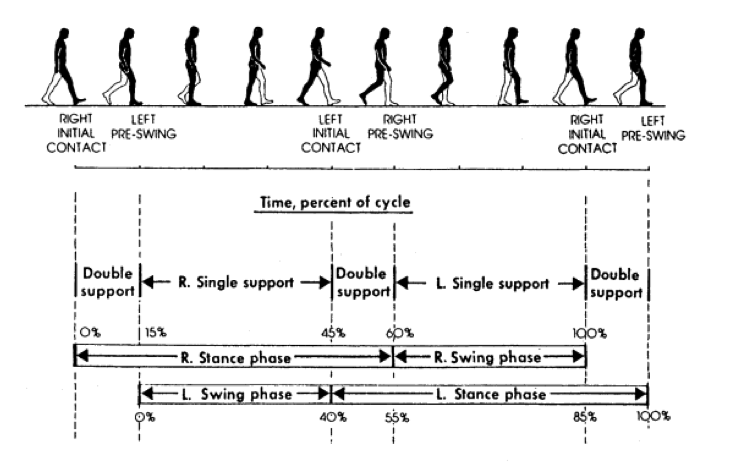
\includegraphics[scale=1.2]{gait_cycle}
  \caption{Time dimensions of the gait cycle. Reprinted from \cite{Inman1981}.}
  \label{fig:gait_cycle}
\end{figure}

\subsection{Gait and Energy Use}

Understanding energy consumption in healthy gait is key to understanding the spatial and temporal dynamics observed during walking. During the gait cycle, three main events occur in which energy is consumed: controlling forward movement during deceleration towards the end of swing phase, shock absorption at heelstrike, and propulsion during push off, when the center of gravity is propelled up and forward\cite{Inman1981}.The least amount of energy required to keep the body in motion would be when the center of mass (located anterior to the second sacral vertebra, midway between both hip joints) moves in a completely straight line, deviating neither up nor down, nor side to side\cite{Inman1981}. This is obviously not the case, and only could be if one's feet were replaced with wheels. Instead, the center of mass (COM) deviates from the straight line in vertical and lateral sinusoidal displacements\cite{Inman1981}. The COM goes through rhythmic vertical displacement as the body moves forward. The highest point occurs at midstance, the lowest point occurs at double support. As weight is transferred from one leg to another, there is a shift of the pelvis to the weight-bearing side. The oscillation of the COM reaches maximum lateral displacement at midstance\cite{Inman1981}.

The seminal paper by Saunders, Inman and Eberhart, which served as the foundation of the description of normal gait for many years, describes six determinants of gait: pelvic rotation, pelvic tilt, stance phase knee flexion, knee and ankle mechanics, and lateral pelvic displacement\cite{SaundersJBInmanVT1953}. Inman and colleagues assert that these components work synergistically to limit excessive displacement of the COM from the smooth sinusoidal trajectory\cite{SaundersJBInmanVT1953}. They infer that since force is the product of mass and acceleration, and acceleration is a function of time, abrupt changes in the direction of the center of motion compel a high expenditure of energy\cite{SaundersJBInmanVT1953}. Thus in translating the COM through a smooth sinusoidal path of low amplitude, the human body conserves energy\cite{SaundersJBInmanVT1953}.

The specific roles of each determinant is outside the scope of this paper, but it is important to note that if one determinant fails, compensatory changes will occur in the others to maintain a normal displacement pattern, in attempt to mitigate energy loss\cite{SaundersJBInmanVT1953}. 

\subsection{Neural Control of Gait}

Walking has generally been considered to be an automatic process involving little or no higher cognitive input\cite{Shik1976}. Our understanding of the automaticity of gait is primarily inferred from experimentation with animal quadropeds. It was demonstrated in the early 1900's that decerebrate cats were able to walk with an essentially normal pattern of stepping\cite{Sherrington1910}. This is corroborated in humans, where infants perform step-like movements if stimulated by peripheral stimuli\cite{Dietz1997}. The demonstration that a simple unpatterned input to the spinal cord can produce complex rhythmic activation patterns led to the principle of central pattern generator (CPG) for the control of locomotion\cite{Mackay-lyons2002}. 

To initiated stepping, incoming sensory information is integrated within multiple, ascending levels of the central nervous system including the spinal cord, brainstem, basal ganglia and thalamic areas \cite{Shik1976, Dietz1997}. Once learned, locomotion is initiated at the level of the supplementary motor area of the frontal lobe and executed by the primary sensorimotor areas, basal ganglia, cerebellum and other brainstem and spinal cord motor centers automatically without input from higher cognition \cite{Shik1976, Dietz1997}. During routine walking, previously learned programs of movement are modified, if necessary, according to a continuous inflow of sensory information from all modalities of perception. This allows for stability of equilibrium, stance and stride\cite{Sheridan2007}. 

Though the suggestion of autonomic control is compelling, evidence using human subjects is inherently difficult to derive, and the locomotive generating capacity of the spinal cord continues to be a subject of debate\cite{Mackay-lyons2002}.

\subsubsection{Gait and Higher Level Neural Input}

Recent research postulates that cognition, executive function, and attention have a more prominent role in the regulation of gait than previously understood\cite{Yogev-Seligmann2008}. Studies with patients with Alzheimer's disease patients have suggested that walking under usual circumstances may require attention and executive function, and changes in cognitive function may contribute to an increased fall risk\cite{Sheridan2007}. Others have shown that impaired executive function is related to decreased walking speed\cite{Persad2008}, increased stride time variability\cite{Allali2008}, increased incidence of falls and decreased performance on complex motor tasks\cite{Yogev-Seligmann2008}. Beyond a better understanding of the physiological control of gait, understanding the relationship between gait variability, stability and executive function can be of great clinical relevance with respect to the early identification of cognitive decline and increased fall risk in older adults\cite{IJmker2012}. This topic is expanded on in Section \ref{sec:var_and_cog} Gait Variability and Cognitive Impairment.

\subsection{Gait Analysis in Clinical Assessment}

Gait analysis is becoming a more widely recognized tool during clinical evaluation. Previous work has shown that changes in gait can be related to physical and cognitive decline\cite{Kluger2008}, due to aging and/or illness \cite{Grabiner2001,Hausdorff2005a}. Common causes of gait abnormalities in older adults include neurological diseases, arthritis and acquired foot deformities\cite{Verghese2002}. Stroke survivors also frequently display gait abnormalities\cite{Patterson2008}. Gait analysis has been evaluated for predicting the risk of developing dementia and, in particular, the risk of developing Alzheimer's disease\cite{Verghese2002}. In addition, gait analysis may help identify and quantify the risk of an elder falling\cite{Toulotte2006}, and it is an essential tool in the treatment and evaluation of cerebral palsy patients\cite{Gage1993}. Gait analysis is also important when fitting prosthetic or orthotic devices, when evaluating the success of an orthopaedic surgery\cite{Aminian2004} or assessing success or failure of a particular rehabilitation program\cite{SantAnna2009}. Gait analysis in a clinical setting may be observational or quantitative in nature, the latter of which is the focus of this review.

\subsubsection{Measurement Tools and Techniques}

Common parameters selected for quantitative gait analysis are spatio-temporal parameters, such as include walking speed, cadence, step length, stance time, swing time, and double support time\cite{Mudge2007}. Parameter measurement may automated or manual. Automated motion laboratories with highly accurate computer-based force and optical tracking sensors (e.g., OptoTrack), instrumented walkways (e.g., GAITRite system), piezodynamometric platforms, and others are used to analyze the motion of body segments to measure characteristic gait parameters\cite{Khusainov2013}. 

Manual measurement may include a series of tests such as Timed Up and Go (TUG)\cite{Khusainov2013}. TUG is a simple mobility test during which the subject is asked to stand up from a chair with an armrest, walk a distance of 3m, turn around and walk back, and sit back down\cite{Herman2011}. The time required to complete the test is measured; if it is below 20 s, the subject is considered to have no mobility issues, and if it is above 30 s, the subject is considered to have serious mobility challenges. Other tools available include the Berg Balance Scores and the Community Balance and Mobility Scales\cite{Steffen2002a}.

There are limitations to both automated and manual approaches. Current automated methods provide accurate results, but they limit examination to a few strides and are constrained to the laboratory setting. These systems are also expensive, must be installed in appropriate rooms, and are complex to operate without specially trained personnel\cite{SantAnna2009}. Manual methods and/or grading scales are inexpensive, but they are prone to individual variation, are harder to systematize and are harder to compare across multiple measurements\cite{Khusainov2013}.

\subsection{Gait Variability}

Like most physiologic signals, measures of gait are not constant, but fluctuate with time and change from one stride to the next, even when environmental and external conditions are fixed\cite{Hausdorff2005}. In healthy adults, these stride-to-stride fluctuations are relatively small and the coefficient of variation of many spatio-temporal parameters is on the order of just a few percent\cite{Gabell1984}. Gait variability was originally considered to represent noise of instrumentation or natural physiologic noise, but recent work has demonstrated that gait variability (stride-to-stride fluctuations) may provide a more discriminative measure of gait performance than routine spatio-temporal measures\cite{Lord2011}.

Gait variability has been proposed to reflect the underlying neural control of gait with demonstrated sensitivity to pathological and ageing processes\cite{Hausdorff2007}. Previous work has found that the timing of gait phases (eg, stance phase, double support phase) in healthy adults is consistent regardless of gender or age\cite{Jansen1982}, suggesting that decline in gait control cannot be attributable to aging alone. Rather, when the systems regulating gait are disturbed as a result of certain diseases, movement control may be impaired leading to increased variability of these gait parameters\cite{Hausdorff2005}.

In an excellent summary paper on gait variability in the \textit{Journal of NeuroEngineering and Rehabilitation}, Jeffrey Hausdorff highlights five important concepts from a body of supporting literature\cite{Hausdorff2005}:

\begin{enumerate}
  \item Gait variability is a quantifiable feature of walking that is altered (both in terms of magnitude and dynamics) in clinically relevant syndromes, such as falling, frailty, and neuro-degenerative disease.
  \item The magnitude of the stride-to-stride fluctuations in stride length and step timing are unaltered in healthy older adults, whereas the dynamics of gait change with healthy aging.
  \item Physiologic factors that affect gait dynamics include neural control, muscle function and postural control; however, more subtle alterations in underlying physiology including cardiovascular changes and mental health may also influence the variability of gait.
  \item Improvements in muscle function and therapeutic interventions are associated with enhanced gait stability, but not always with more conventional measures of average gait velocity or cadence.
  \item Gait instability measures apparently predict falls in idiopathic elderly fallers and other populations who share an increased fall risk.
\end{enumerate}

Three decades ago, Gabell and Nayak speculated that stride time variability reflects gait timing mechanisms and the pattern generator of gait, while variability of support time and step width more closely reflect balance control\cite{Gabell1984}. Though no consensus has been reached, gait variability may serve as a sensitive and clinically relevant parameter in the evaluation of mobility, fall risk, the response to therapeutic interventions and cognitive function\cite{Hausdorff2005}.

\subsubsection{Spatial Variability, Temporal Variability and the Relationship with Gait Speed}

When all other variables are kept constant, studies in young adults have demonstrated a ``U-shaped'' relationship between gait speed (in terms of stride length and/or cadence) and measures of gait variability\cite{Hausdorff2005}. In other words, variability is observed most commonly when walking speed is outside the bounds of a person's usual cadence. When investigating gait and the factors that influence variability, it is important to take into account the possibility that any observed group differences or responses to intervention are simply a result of changes in gait speed\cite{Hausdorff2005}. There is evidence that modifications to stride length will affect spatial variability\cite{Sekiya1997} and modifications to stride frequency will affect  temporal variability\cite{Maruyama1992}.

Most often assessed as separate variables, Danion and colleagues\cite{Danion2003} addressed spatial and temporal aspects of gait variability concurrently. At a general level, they found that across all experimental conditions, spatial and temporal variability increased or decreased in concert, and regression analysis confirmed a significant relationship between the two variables\cite{Danion2003}. Figure \ref{fig:temp_spat_variability}, shows variability of the stride as a function of stride frequency and stride amplitude. Variability was reported as standard deviation ($SD$, absolute units) and coefficients of variation ($CV = SD/Mean$, relative units) at varying levels of stride length (2A, 2C) and stride frequency (2B, 2D). Stride frequency showed the characteristic U-shaped curve, where intermediate frequency lead to minimal temporal and spatial variability. Shorter stride lengths lead to greater temporal and spatial variability\cite{Danion2003}. Important caveats to consider are that the study only included eight subjects, all of whom were healthy young adults.

\begin{figure}[H]
  \centering
    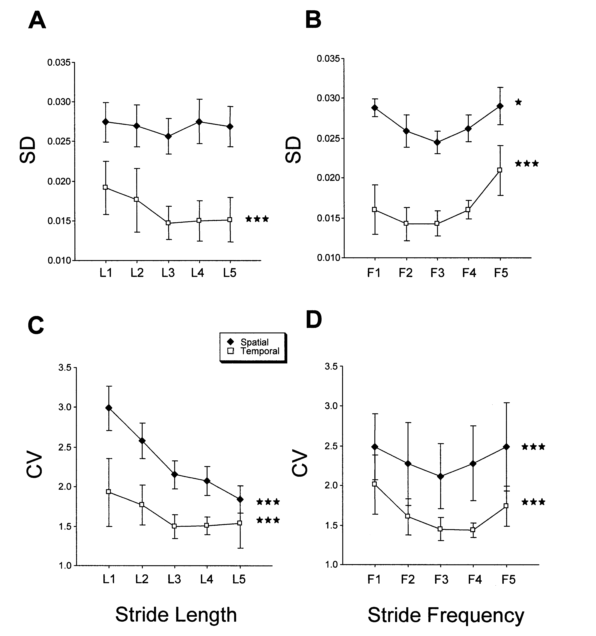
\includegraphics[scale=0.7]{temp_spat_variability}
  \caption{Variability of the stride as a function of stride frequency and stride amplitude. Data are averaged across experimental conditions. The effects of stride frequency (B, D) and length (A, C) are presented on separate columns (respectively, left and right). Variability is either expressed by the $SD$ (top row) or by the coefficient of variation ($CV$, bottom row). $SD$'s are expressed in meters for stride length, and in Hertz for stride frequency. The error bars represent the $SD$ across the five experimental conditions. Stars indicate when the difference between experimental conditions is significant (* for \textit{P} $<$ 0.05, and *** for \textit{P} $<$ 0.001). Reprinted from \cite{Danion2003}.}
  \label{fig:temp_spat_variability}
\end{figure}

\subsubsection{Gait Variability and Cognitive Impairment}
\label{sec:var_and_cog}

As previously described, increasing evidence from clinical practice, epidemiological studies, and clinical trials shows that gait and cognition are inter-related in older adults\cite{Montero-Odasso2013}. Early disturbances in cognitive processes such as attention, executive function, and working memory are with slower gait and gait instability during single and dual-task testing, and that these cognitive disturbances may assist in the prediction of future mobility loss, falls, and progression to dementia\cite{Montero-Odasso2013}. 

Quantification of gait instability through gait variability is receiving growing attention in the literature. The variability of several spatio-temporal parameters have been studied, with stride to stride fluctuations in gait cycle timing (e.g., stride time) being the most widely reported\cite{Montero-Odasso2013}. It has been suggested that stride time reflects one of the final pathways of the outcomes regulated by the central nervous system\cite{Montero-Odasso2013}. Stride time variability is becoming a relevant marker of gait stability, both in research and clinical practical, as it can be measured easily and robustly\cite{Hausdorff2005}. The general assumption is that there is an inverse association between stride time variability and gait stability\cite{Montero-Odasso2013}. Low stride time variability reflects automatic processes that require minimal higher cortical input, and is associated with efficient and safe gait patterns\cite{Hausdorff2005}.

Deficits in cognitive function and mobility co-exist in older adults even in the early stages of aging\cite{Montero-Odasso2013}. Older people with mild cognitive impairment syndrome (MCI) may have impairments in either memory (amnestic) or non-memory (non-amnestic) domains\cite{Yamada2011} as well as impairments in fine and complex motor skills, equilibrium, and limb coordination\cite{Montero-Odasso2013}. One study that included amnestic and non-amnestic MCI participants found that low performance in three related cognitive domains (i.e., attention, executive function, and working memory) was associated with slowing of gait velocity specifically under dual-task conditions, suggesting that these specific cognitive domains are relevant for maintaining a normal gait pattern in the presence of a cognitive load\cite{Montero-Odasso2009}. Another study found that increased variability of time-related gait parameters were significantly different under dual-task testing in older adults with MCI compared to age-matched normal controls, but less affected than in people with mild Alzheimer's disease (AD) \cite{Muir2012a} The same group compared the effect of dual-task of different complexity between cognitively normal controls and older adults with MCI\cite{Montero-Odasso2012} A significant dual-task cognitive status interaction was found for gait variability, but not for gait velocity, further demonstrating that gait variability may be especially sensitive to dual-tasking and to the complexity of the task given\cite{Montero-Odasso2013}. These findings are in line with the view that the regulation of variability is normally automated and requires minimal cognitive input. However, when automaticity is impaired (e.g., in the presence of pathology), cognitive tasks affect gait variability. A summary of studies that examined gait variability and cognitive function is shown in Table~\ref{tab:gait_cog_table}.

\begin{table}[!htb]

\begin{adjustbox}{max width=\textwidth}
  \begin{tabular}{| l | p{4cm} | p{4cm} | p{7cm} |}

    \hline
    \textbf{First author (year)} & \textbf{Patient population} & \textbf{Measurement tool} & \textbf{Findings} \\ \hline
    
    Hausdorff (2003)\cite{Hausdorff2003} & Parkinson's & Force-sensitive insoles & Gait variability increased when cognitively challenged. \\ \hline
    
    Sheridan (2003)\cite{Sheridan2003} & Older adults with probable AD & Force-sensitive insoles  & Subjects walked with greater gait variability than older adults without AD at normal pace. Gait variability increased with dual-task walking. The effect on gait variability was larger than the effect on gait speed. Executive function were significantly associated with the increased gait variability that occurred when walking with divided attention but not with gait speed or usual, single-task walking measures of gait. \\ \hline
    
    Yogev (2005)\cite{Yogev2005} & Parkinson's vs. healthy controls & Force-sensitive insoles & Gait variability increased with cognitive loading, but was not related to Mini-Mental Status Exam scores, to memory, or to information processing abilities. \\ \hline
    
    Hausdorff (2005)\cite{Hausdorff2005b} & Healthy older adults & Force-sensitive insoles & Gait variability was strongly dependent on executive function, but not on memory. \\ \hline
    
        Allali (2008)\cite{Allali2008} & Older adults with AD vs. healthy controls & GAITRite System & Stride time variability increased while performing dual tasking. Stride time variability was higher in demented subjects with impaired executive function (IEF) when compared to nondemented subjects, but not when compared to the demented subjects without IEF. \\ \hline
        
    Muir (2011)\cite{Muir2012a} & Older adults with AD \& MCI & GAITRite System & Significant differences of decreasing velocity, increasing stride time and increasing stride time variability were found under dual-task testing for people with MCI and AD. \\ \hline
    
    Beauchet (2013)\cite{Beauchet2013} & Older adults with AD \& MCI & GAITRite System & Stride time variability was associated with MCI status at fast-pace walking speed. \\ \hline
    
        Montero-Odasso (2014)\cite{Montero-Odasso2014} & Older adults with MCI and healthy controls & GAITRite System & MCI participants showed higher stride time variability than no-MCI in all conditions with a statistically significant difference for simple and dual-task counting gait. \\ \hline

    
  \end{tabular}
\end{adjustbox}
\caption{Gait Variability and Cognitive Function}\label{tab:gait_cog_table}
\end{table}

\pagebreak

\chapter{Gait Analysis Using Wearable Sensors}

The utility of a system that is inexpensive, unobtrusive, easy-to-use, and allows for quantitative analysis of gait patterns outside the laboratory has been well argued in the literature\cite{Tao2012, SantAnna2009, Patel2012, Itoh2008, Malaric2010, Godfrey2015}. The common themes that arise is that characterizing gait within the laboratory setting may not accurately reflect a patient's walking pattern in the home environment, the length of data collection is limited, and access to a sophisticated gait laboratory is limiting. Sensor-based approaches to gait assessment are being increasingly adopted as they facilitate quantitative and repeatable analysis\cite{Khusainov2013}. With the increasing popularity of smartphones, wearable devices, and internet-enabled objects, there is an opportunity to leverage existing technology to provide unprecedented accessibility to diagnostic tools.

\section{Data Acquisition}

Gait analysis has been implemented using different types of motion sensors and systems, such as the accelerometer, gyroscope, magnetoresistive sensors, flexible goniometer, electromagnetic tracking system (ETS), sensing fabric, force sensor, and sensors for electromyography (EMG) \cite{Tao2012}. Extensive adoption of smartphones and body-worn electronics (``wearables'') makes accelerometers, gyroscopes and magnetoresistive sensors most attractive to consider because they are embedded into many of these devices. This is in part due to enhancements in micro-electro-mechanical systems (MEMS) technology which has enabled the manufacture of miniaturized, low power, low cost components\cite{SantAnna2009}. The basic principles and features of these sensors are described.

\subsection{Accelerometers}

An accelerometer is a type of inertial sensor that can measure acceleration along its sensitive axis\cite{Tao2012}. The common operation principle of accelerometers is based on a mechanical sensing element that comprises a proof mass attached to a mechanical suspension system, with respect to a reference frame\cite{Tao2012}. The mass proof can be forced to deflect by the inertial force because of acceleration or gravity according to Newton's Second Law ($force = mass \times acceleration$). Based on this principle, the acceleration can be measured electrically using the physical changes in the displacement of the proof mass, with respect to the reference frame\cite{Tao2012}.

\subsection{Gyroscopes}

A gyroscope is an angular velocity sensor. The micromachined gyroscope is based on the concept of measuring the Coriolis force, which is an apparent force proportional to the angular rate of rotation in a rotating reference frame\cite{Tao2012}. By detecting the linear motion from the Coriolis effort and performing an integration of the gyroscopic signal, the angular rate can be obtained\cite{Tao2012}. A gyroscope can be applied for gait analysis by identifying initial and final contact with the floor (tail ends of the stance phase) by measuring the angular rate\cite{Catalfamo2010}.

\subsection{Magnetoresistive Sensors}

Magnetoresistive sensors are based on the magnetoresistive effect\cite{Tao2012}. If a magnetic flux (magnetic field) is not applied, the current flows straight through the InSb plate within the sensor. However, if a magnetic flux is applied, a Lorentz force proportional to the magnetic flux density will deflect the current path. As the current path is deflected, the current flows through the plate for a longer distance, causing the resistance to be increased\cite{Tao2012}. That is, the magnetoresistive effect refers to the change in the resistivity of a current carrying ferromagnetic material resulting from a magnetic field, with the resistance change proportional to the tilt angle in relation to the magnetic field direction\cite{Graham2004}. Based on this magnetoresistive effect, magnetoresistive sensors can estimate changes in the orientation of a body segment in relation to the magnetic North or the vertical axis in the gait analysis\cite{Choi2008}. Such sensors can provide information that cannot be determined by accelerometers or the integration of gyroscope signals\cite{Tao2012}.

\section{Signal Processing and Data Analysis}

Quantitative gait analysis requires raw sensor acquisition, signal processing and data analysis. Review of the literature reveals variation in approaches. Sensor data processing and analysis stages commonly include pre-processing (e.g., filtering), segmentation, feature extraction and feature selection\cite{Khusainov2013}. Acquired sensor measurements are often pre-processed to remove noise and artefacts, because signals are easily corrupted by instrumentation noise, random noise, electric and magnetic noise\cite{Khusainov2013}.

\subsection{Filtering}

Typical filters for acceleration signals include median, Butterworth low-pass, discrete wavelet package shrinkage and Kalman filters\cite{Wang2011}. The effects of these filters in terms of signal-to-noise ratio and correlation coefficient on 3D accelerometer human mobility data were investigated in\cite{Wang2011}, and the following findings reported:

\begin{enumerate}
  \item Kalman filters showed the largest SNR and R values, followed by median filters, discrete wavelet package shrinkage, and then Butterworth low-pass filters.
  \item Performance of Butterworth low-pass filters marginally improved over that of Kalman filters after correcting waveform delay for Butterworth low-pass filters.
  \item Performance of median filters is related to their window length.
  \item Decomposition level influenced real-time performance of discrete wavelet package shrinkage.
  \item Filter order and cut-off frequency, if not properly selected, could result in large waveform delay for Butterworth low-pass filters.
\end{enumerate}

\subsection{Feature Extraction}

Different applications require the extraction of certain sets of discriminatory features from the sensor datasets using unique metrics\cite{Khusainov2013}. The metric used depends on the required features and representation domain of the dataset (time, frequency, or discrete)\cite{Khusainov2013}. 

Analysis of signals in the time domain deals mainly with two dimensions: amplitude and time, which facilitate the extraction of features using statistical metrics including mean, median, variance, standard deviation, minimum, maximum, range, Root Mean Square, correlation, and cross-correlation\cite{Figo2010}. Other time domain metrics include sample differences, angle (tilt angle), zero-crossings, Signal Magnitude Average, and Signal Magnitude Vector\cite{Figo2010}.

Accelerometer data in the frequency domain have two components: DC and AC. The DC component constitutes the first coefficient in the spectral representation of the signal and its value is often much larger than the remaining spectral coefficients, while the AC component is the dominant frequency component\cite{Figo2010}. These components are the basis for the extraction of most of the time and frequency domain features. Accelerometer signal can also be transformed into strings of discrete symbols (discrete domain representation)\cite{Figo2010}. String represented data can be analyzed for string similarity and pattern discovery using exact or approximate matching and edit distance techniques such as Euclidean-related distances\cite{Figo2010}.

\subsection{Processing Location}

The processing location is another important factor. It may be on-board the monitoring device, or it may be transmitted to base station for processing (or both)\cite{Khusainov2013}. The computational costs, storage requirements, and precision (data representation format) of the algorithm must be assessed to determine suitability for on-board versus base station processing\cite{Khusainov2013}. On-board sensor data processing poses greater challenges due to hardware constraints, which limit the amount of data that can be buffered, the robustness of classification algorithms, and the range of events that can be classified\cite{Karantonis2006}. Figo and colleagues\cite{Figo2010} investigated processing techniques in the time, frequency and discrete domains and report their associated computational costs.

\section{Usability Considerations}

The following requirements are based on anecdotal feedback from clinicians and researchers at the University of Toronto, Bridgepoint Hospital, and Toronto Rehabilitation Institute. It builds off of similar requirements and learnings from a prototype developed and evaluated by Phil Lam and Anita Ko in the Knowledge Media and Design Lab\cite{Lam2012, Ko2012}:

\begin{table}[!h]

%\begin{adjustbox}{max width=\textwidth}
  \begin{tabular}{p{\textwidth}}

	\textbf{Hardware Requirements (sensor package)}    \\ \hline 
	Battery must last at least 24 hours \\ \hline
	Sensor should collect data at an appropriate frequency to minimize power-consumption and data-overload \\ \hline
	Sensor should be wireless \\ \hline
	Sensor should be easy to recharge \\ \\ 
	\textbf{Interface Requirements (collection and analysis of data)}    \\ \hline 
	Easy to see when the sensor is turned on, turned off, and recording data \\ \hline
	Easy to download the data \\ \hline
	Easy to process the data \\ \hline
	Easy to visualize the results in a summarized manner \\ \hline
	Easy to choose summary measures to report \\ \hline
	Appropriate visualization for patients, clinicians and non-medical caregivers \\ \\
	
	\textbf{User Requirements (Patients)} \\ \hline 
	Conspicuous (non-obtrusive) \\ \hline 
	Non-distracting \\ \hline 
	Comfortable to wear \\ \hline 
	Easy to put on \\ \hline 
	Meaningful feedback/visualization of gait data \\ \\
	
	\textbf{User Requirements (Clinicians)}  \\ \hline 
	Clinical relevant metric and measurement scale \\ \hline 
	Assessment of metric against historical data (population-wide and personal) \\ \hline 
	Does not interfere considerably with current clinical workflow \\ \hline 
	Does not negatively influence patient-clinician interaction \\ \hline 
	Is not labor intensive to collect or process data \\ \\
	
	\textbf{User Requirements (Non-medical caregivers)} \\ \hline
	Meaningful feedback/visualization of gait data \\ \hline 
	Assessment of metric against historical data (personal) \\ \hline 
	
  \end{tabular}
 % \end{adjustbox}
\end{table}

\subsubsection{Progress to Date}

A simple data-collection tool is currently being developed. The tool consists of a LightBlue Bean\footnote{http://legacy.punchthrough.com/bean/} containing a 3-axis accelerometer (Figure \ref{fig:bean}), and an Android\footnote{https://www.android.com/} application for data collection (Figure \ref{fig:app_screenshot}). Data analysis is currently done using MATLAB\footnote{www.mathworks.com/products/matlab/}, but will be integrated into the Android application in the future. \\

\begin{figure}[h]
    \centering
    \begin{subfigure}[b]{0.4\textwidth}
        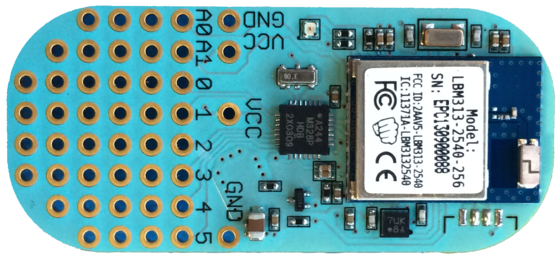
\includegraphics[width=\textwidth]{bean}
        \caption{LightBlue Bean}
        \label{fig:bean}
    \end{subfigure}
    \hspace{3cm}
    \begin{subfigure}[b]{0.3\textwidth}
        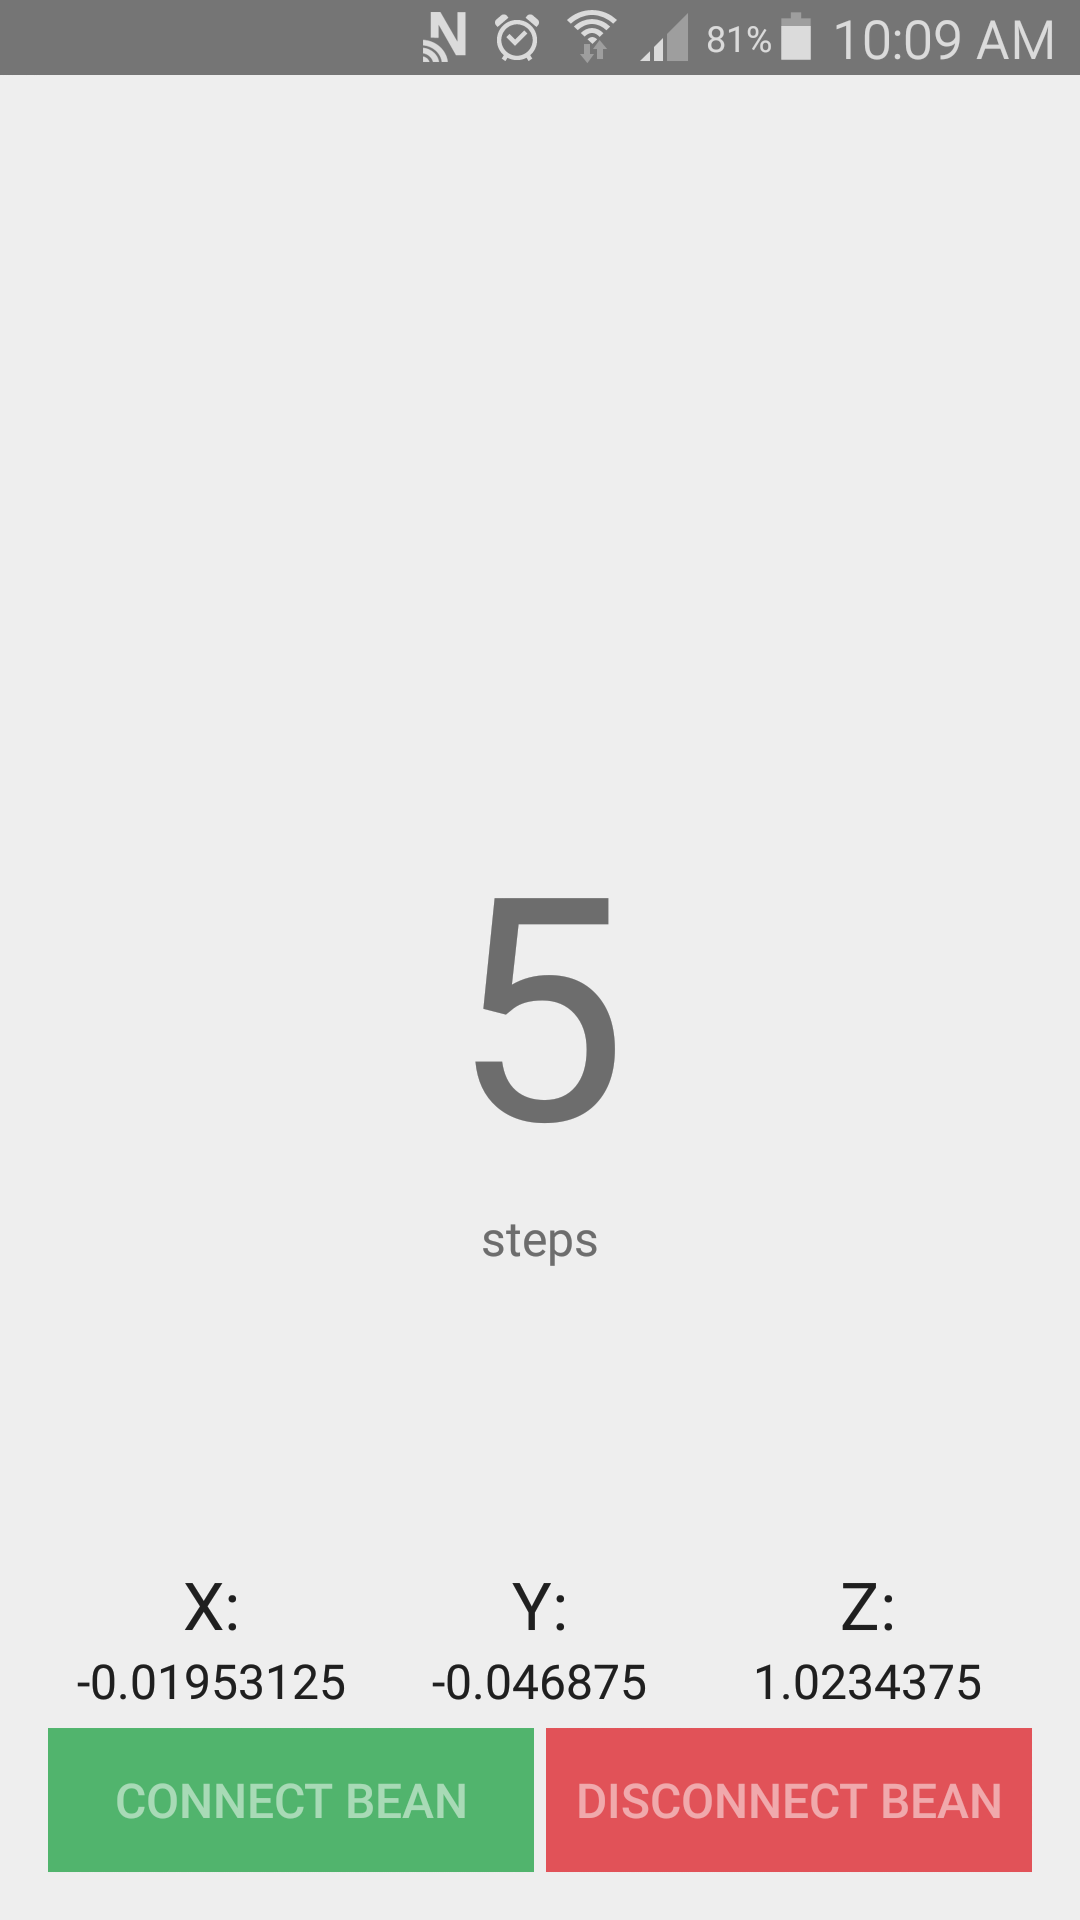
\includegraphics[width=\textwidth]{app_screenshot}
        \caption{Android application}
        \label{fig:app_screenshot}
    \end{subfigure}
        \caption{Hardware and software under development.}\label{fig:progress}
\end{figure}

The LightBlue Bean (the ``Bean") is a low energy Bluetooth Arduino microcontroller. Using Bluetooth 4.0, it is programmed wirelessly, runs on a coin cell battery, and is easily integrated with smartphone applications. It is small and lightweight, which makes it a more unobtrusive monitoring device. However, it may not be the ideal hardware for this project because it does not provide a fast enough sampling rate for detection of certain features of gait.

The Android application is being developed using Android Studio\footnote{http://developer.android.com/sdk/index.html}, an integrated development environment for Android applications. This was chosen based on the availability of low-cost mobile phones, tablets and wearable devices that run on the Android operating system\footnote{And the fact that the author doesn't have an iPhone.}.

Robust filtering, segmentation and feature analysis has not yet been implemented. However, proof-of-concept for simple detection of a gait event has been developed. Accelerometer data was collected with the Bean mounted on the ankle. The Android application saves the raw values to a csv file which is manually transferred to a laptop computer for analysis (Figure \ref{fig:raw_data}). The data is smoothed with a moving average filter with a window of 2 samples. This is a low-pass filter to smooth out short-term fluctuations and highlight the gait cycles. Local maximas are calculated to identify a step has occurred. Mean stride time and the variance of the stride time can be calculated (Figure \ref{fig:smooth_max}).

\begin{figure}[!p]
\begin{adjustbox}{varwidth=1.2\textwidth,center}
\begin{subfigure}[center]{\textwidth}
  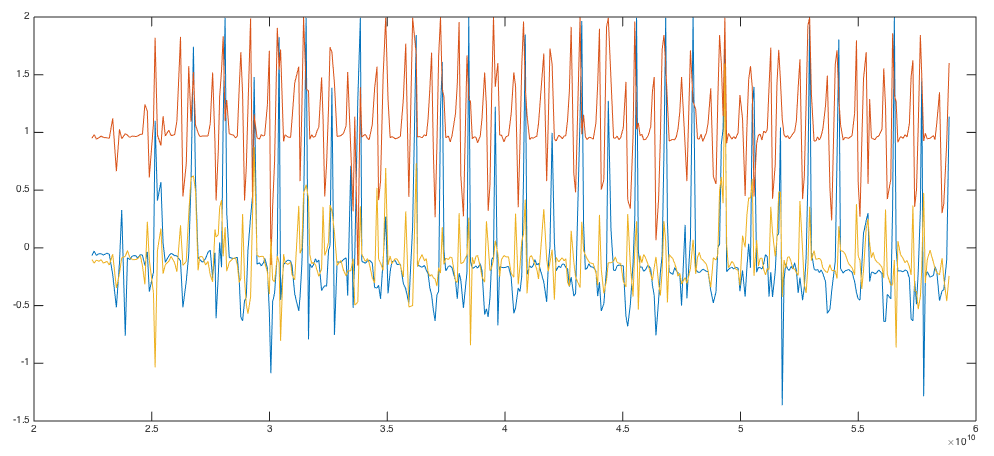
\includegraphics[width=20cm]{xyz_raw}
  \caption{Raw accelerometer data from x, y and z axes}
  \label{fig:raw_data}
\end{subfigure}

\begin{subfigure}[center]{\textwidth}
 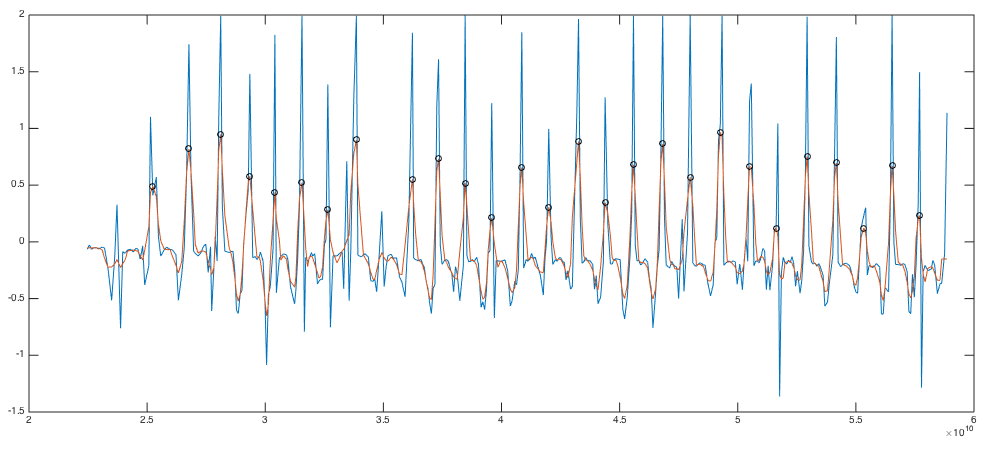
\includegraphics[width=20cm]{x_smooth_maximas}
  \caption{Smoothing and identification of gait events}
  \label{fig:smooth_max}
  \end{subfigure}
   \end{adjustbox}
   \caption{Accelerometer data plotted using MATLAB}\label{fig:matlab_graphs}
\end{figure}

\pagebreak

\section*{Conclusions}
\addcontentsline{toc}{section}{\textsc{\textbf{Conclusion and progress to date}}} % add to TOC


Neuropsychological status plays an important role in gait instability, but the relationship has not yet been quantitatively defined. As well, available tools are not appropriately designed for practical use by clinical caregivers. The ability to easily monitor changes in gait dynamics may help to prospectively identify decline in cognitive function, prompting earlier interventions that improve quality of life for older adults.

In this thesis research, I seek to evaluate if gait variability can be reliably quantified to indicate underlying degeneration of neurological motor control, and associated cognitive impairment. The outcome of this research is expected to be an understanding of how gait analyses may predict cognitive impairment, and the development of functional clinical tools for implementing simplified gait analysis outside a controlled laboratory.


\pagebreak
\bibliography{Gait}
\addcontentsline{toc}{section}{\textsc{\textbf{References}}} % add to TOC


\end{document}  